
\newpage
\section{Webots-Simulationsumgebung}
  Hier wird die in Webots realisierte Simulationsumgebung vorgestellt, die als zentraler Versuchsstand für Entwurf, Parametrierung
  und Evaluation der kombinierten Regelung des selbstbalancierenden Fahrrads dient. Ziel ist es, ein reproduzierbares und sicheres  
  Testbett zu schaffen, in dem das physikalische Fahrverhalten, die sensorgeführte Pfadverfolgung sowie die Kopplung von schneller
  Balance-Regelung und langsamer Vision-/Trajektorienplanung unter kontrollierten Bedingungen untersucht werden können. Webots
  bietet dafür eine deterministische Dynamiksimulation auf Basis von ODE, eine hierarchische Szenenbeschreibung und eine klare
  Trennung von Geometrie, Physik, Sensorik, Aktuatorik und Controllern – Eigenschaften, die systematische Parameterstudien,
  Logging und automatisierte Auswertung wesentlich erleichtern \cite{cyberbotics2025}.

  Das Kapitel ist wie folgt strukturiert: Zunächst wird ein Überblick über Webots und die genutzten Kernfunktionen gegeben.
  Anschließend wird die konkrete Szenenstruktur der Weltdatei erläutert, einschließlich globaler Simulationsparameter und
  der Organisation der Knoten. Darauf aufbauend folgt die Beschreibung des Fahrradmodells mit seinen Gelenken, Kontakt- und
  Masseneigenschaften sowie der eingesetzten Sensoren und Aktuatoren. Abschließend werden die Controller-Prozesse und deren
  Interaktion skizziert sowie die angebundene GUI bzw. Auswertepfade beschrieben. Diese Gliederung macht transparent, wie
  ausgehend von einem konsistenten physikalischen Modell die Regelungsalgorithmen iterativ entwickelt, validiert und
  für den späteren Transfer auf den Realprototyp vorbereitet werden.



  \subsection{Überblick}
  Webots ist ein frei verfügbares, quelloffenes und plattformunabhängiges Robotik Simulationsprogramm, das seit 1998 kontinuierlich 
  gepflegt wird und in Forschung, Lehre und Industrie breite Anwendung findet \cite{michel2004,cyberbotics2025}. Es kombiniert eine 
  moderne Qt\-Benutzeroberfläche mit einer Mehrkörper\-Dynamiksimulation auf Basis der \emph{Open Dynamics Engine} (ODE) sowie einer 
  OpenGL\-gestützten Rendering\-Pipeline. Dadurch lassen sich fotorealistische 3D\-Szenen mit deterministischem Integrationsschema und 
  feingranularer Kontrolle der Simulationszeit schrittgenau ausführen \cite{cyberbotics2025}.

  Kern des Webots\-Modells ist die hierarchische Szenenrepräsentation in \textit{World}\-Dateien 
  (\texttt{*.wbt}; VRML\-basiert). 
  Eine Welt kapselt globale Parameter (z.\,B.\ Zeitauflösung, Kontakt\- und Reibungsmodelle), Umgebungsobjekte (Boden, Licht, Hintergrund) 
  sowie Roboterknoten mit Sensorik, Aktuatorik und Masseneigenschaften. Geräte (z.\,B.\ Kamera, IMU, Lidar, \texttt{RotationalMotor}) 
  sind als Nodes mit klar definierten Schnittstellen realisiert; ihre Parameter (Auflösung, Bildfrequenz, Dämpfung, Grenzwerte) sind 
  reproduzierbar konfigurierbar. Controller laufen als getrennte Prozesse in C/C++, Python, Java oder MATLAB und kommunizieren zur Laufzeit 
  über wohldefinierte APIs mit der Simulationswelt; mittels ROS~2\-Bridge ist zudem eine Einbettung in verteilte Robotik\-Stacks möglich 
  \cite{gupta2023,cyberbotics2025}. Eine spezielle \emph{Supervisor}\-API erlaubt höherwertige Eingriffe (Positionsreset, automatisiertes 
  Logging, Metrik\-Auswertung) und bildet die Grundlage für reproduzierbare Benchmarking\-Pipelines \cite{cyberbotics2025}.

  Für regelungsorientierte Studien bietet Webots drei Eigenschaften, die in dieser Arbeit zentral sind: (i) \emph{Determinismus} durch festen 
  Zeitschritt und explizite Integrationsreihenfolge, was faire Parameterstudien ermöglicht; (ii) \emph{Modularität} durch die Trennung von 
  Geometrie, Physik, Sensorik/Aktuatorik und Controllern, wodurch Varianten (z.\,B.\ Reibungskoeffizienten, Trägheiten, Abtastraten) isoliert 
  untersucht werden können; (iii) \emph{Automatisierbarkeit} über den Supervisor, u.\,a.\ für Szenario\-Resets, Störgrößeninjizierung, Batch\-Runs 
  und standardisierte Ergebnisberichte \cite{cyberbotics2025}.

  Relevanz für \emph{fahrdynamische Einspurfahrzeuge}: In jüngeren Arbeiten wird Webots gezielt zur Simulation von Fahrrädern und Motorrädern 
  eingesetzt. Das Open\-Source\-Add\-on \emph{WeBikes} erweitert Webots um ein konfigurierbares, physikalisch fundiertes Einspurfahrzeugmodell 
  (Geometrie, Masseverteilung, Reifenkontakt, Steuerkinematik) und demonstriert, dass typische Phänomene wie Selbststabilisierung, Lenkdynamik 
  und Kurvenfahrt reproduzierbar abgebildet werden können \cite{li2024webikes}. Damit wird ein freier, reproduzierbarer Vergleich zu Spezialwerkzeugen 
  ermöglicht und eine Brücke zwischen Regelungsentwurf (z.\,B.\ Balanceregelung, MPC\-Trajektorienplanung) und virtuellen Fahrversuchen geschlagen. 
  Über den gleichen Mechanismus nutzen weitere Studien Webots als Digital\-Twin\-Plattform für komplexe, materialabhängige Systeme (z.\,B.\ weiche Greifer),
   was die Übertragbarkeit auf neuartige Robotertypen unterstreicht \cite{hadi2024softgripper}.

  Für diese Arbeit ist Webots folglich ein geeignetes Testbett, um die Kopplung einer schnellen Balance\-Regelung (PID, \(\approx\)kHz\-Skala) mit einer 
  langsameren vision\- bzw.\ modellprädiktiven Pfadführung (tens of Hz) systematisch zu entwerfen, zu parametrieren und zu evaluieren. Die klare Trennung 
  der Subsysteme (Physik, Sensorik, Controller) erlaubt ablation\-artige Studien (z.\,B.\ Variation von Zeitschritt/Reibung, Sensorausfall, Verzögerungen), 
  während die Supervisor\-Schnittstelle reproduzierbare Kampagnen mit konsistentem Logging unterstützt \cite{cyberbotics2025}.




  \subsection{Struktur der Simulationsumgebung}
  Die verwendete Simulationsumgebung basiert auf Webots und damit auf einer hierarchisch organisierten Szenenbeschreibung 
  im VRML-Format. Eine \texttt{.wbt}-Datei kapselt sämtliche Entitäten der virtuellen Welt – von globalen 
  Parametern (Zeitauflösung, Kontaktmodelle) über Umgebungsobjekte (Boden, Hintergrund, Lichtquellen) bis 
  hin zu Robotern mitsamt deren Sensorik, Aktuatorik und Controllern \cite{cyberbotics2025,gupta2023}. Jeder Knoten (Node) kann wiederum 
  Unterknoten besitzen, sodass sich komplexe Systeme modular aus standardisierten Bausteinen zusammensetzen 
  lassen. Für die vorliegende Arbeit ist diese Hierarchie entscheidend, weil sie erlaubt, (i) das physikalische 
  Verhalten des Fahrrads getrennt von (ii) der Szenengeometrie und (iii) den übergeordneten Reglerprozessen 
  zu modellieren. Änderungen an einem Teilbereich – etwa an den Reibungsparametern der Reifen oder an der 
  Position einer Kamera – bleiben somit lokal und beeinträchtigen die übrigen Komponenten nicht.
  
  Ausgangspunkt der Welt ist eine rechteckige Bodenarena mit texturierter Fahrbahnoberfläche, die als Referenzstrecke 
  für die visuelle Spurführung dient. Globale Kontakt- und Reibungsparameter sind hier definiert, um das Zusammenspiel 
  zwischen Reifen und Untergrund konsistent zu halten. Ein fester Zeitschritt im Millisekundenbereich stellt sicher, 
  dass sowohl die Balancebewegungen des Fahrrads als auch die Bildverarbeitungsschleifen deterministisch und in Echtzeit 
  simuliert werden können \cite{cyberbotics2025}. Die Kameraperspektive des Betrachters (Viewpoint) folgt dem Fahrrad aus erhöhter Position, 
  was die visuelle Analyse der Fahrmanöver während der Versuche erleichtert.
  
  Das zentrale Element der Szene ist der Roboterknoten \emph{BICYCLE}, der das selbstbalancierende Fahrrad repräsentiert. 
  Sein Geometriemodell wurde aus CAD-Daten übernommen und mit vereinfachten Kollisionsvolumina (Boxen und Zylinder) hinterlegt, 
  um die Physiksimulation effizient zu halten. Die Massen- und Trägheitsparameter der Baugruppen (Rahmen, Räder, Gabel) sind 
  explizit angegeben, sodass die Dynamik – insbesondere Roll- und Nickbewegungen – realitätsnah nachgebildet wird. Bewegliche 
  Komponenten sind über Hinge-Joints angebunden: Das Hinterrad wird über einen Rotationsmotor für den Vortrieb angesteuert, 
  die Lenkbewegung des Vorderrads erfolgt über ein zweites Gelenk mit eigenem Servomotor. Ergänzend existiert ein Kurbel-/Pedal-Gelenk, 
  das in erster Linie der geometrischen Vollständigkeit und nicht der Antriebserzeugung dient. Zur Zustandserfassung sind 
  Sensorschnittstellen integriert: Eine Inertialmesseinheit (IMU) liefert dem Balance-Regler fortlaufend Orientierung und 
  Rollwinkel \cite{bno055}; eine am Fahrrad montierte Kamera kann genutzt werden, um on-board visuelle Informationen 
  auszuwerten. Ein Display-Modul steht optional für Debug- oder Visualisierungszwecke zur Verfügung. Die Kommunikation 
  zwischen Fahrrad und übergeordnetem Regler erfolgt über ein Paar aus \texttt{Emitter} und \texttt{Receiver}, die einen 
  leichten, paketbasierten Nachrichtenaustausch innerhalb von Webots ermöglichen.
  
  Übergeordnet ist ein \emph{Supervisor}-Knoten angelegt. Dieser spezielle Robotertyp besitzt in Webots weitreichende 
  Eingriffsmöglichkeiten auf Welt-Ebene (z.\,B. Position-Reset, Logging, automatisierte Auswertung) und dient hier als 
  externe Beobachter- und Steuerinstanz. Der Supervisor trägt eine statisch in der Szene platzierte Kamera, die die Fahrbahn 
  aus einer globalen Perspektive erfasst. Auf Basis dieser Bilder führt der Python-basierte Vision-Controller eine 
  Spurdetektion (YOLO) durch und berechnet über ein modellprädiktives Regelungsverfahren (MPC) Lenksollwerte bzw.\ Trajektorien. 
  Diese Kommandos werden per Funkkanal (Emitter) an den Balance-Controller des Fahrrads übertragen, der sie in konkrete 
  Motorbefehle umsetzt. Umgekehrt sendet das Fahrrad Statusdaten zurück, die der Supervisor für Evaluations- und Loggingzwecke 
  speichert. Dieses Zusammenspiel zweier Controller-Prozesse – ein echtzeitnaher PID-Regler in C auf Roboterseite und ein 
  bildverarbeitungsgetriebener MPC-Regler in Python auf Supervisorebene – bildet die Kernstruktur der kombinierten Regelung.
  
  Die gewählte Struktur der Simulationsumgebung verfolgt zwei Ziele: Erstens ermöglicht sie reproduzierbare und sichere 
  Experimente in verschiedensten Fahrszenarien (Geradeausfahrt mit Störimpuls, Slalomkurse, Kurvenfahrten mit Steigung), 
  ohne das reale Hardware-Risiko des Umkippens oder der Beschädigung einzugehen. Zweitens gestattet die klare Trennung von 
  physikalischem Modell, Sensorebene und Reglerlogik eine gezielte Variation einzelner Parameter (z.\,B. Reibung, Zeitschritt, 
  Bildauflösung), um deren Einfluss auf die Gesamtperformance systematisch zu untersuchen. Webots fungiert damit als flexibles 
  Testbett, in dem sowohl Balance- als auch Spurführungsalgorithmen iterativ entwickelt, validiert und optimiert werden können, 
  bevor sie auf den realen Prototyp übertragen werden.
  \pdfcomment{Bild der Struktur der Simulationsumgebung anzeigens}





  \newpage



  \subsection{Das Fahrradmodell}
  \begin{wrapfigure}{r}{0.42\textwidth} % r=rechts, l=links
    \vspace{-0.8\baselineskip}          % optional: nach Bedarf anpassen
    \centering
    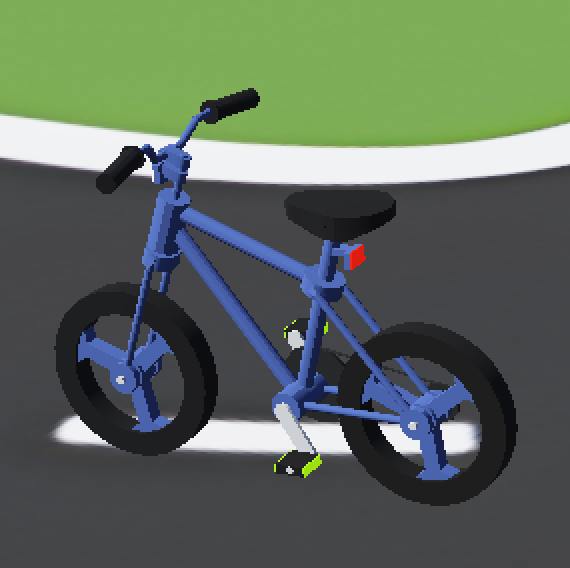
\includegraphics[width=\linewidth]{figures/bicycle.png}
    \caption{Das Fahrradmodell in Webots.}
    \label{fig:bicycle}
  \end{wrapfigure}

  Das folgende Kapitel führt in das in Webots implementierte Fahrradmodell ein, 
  wie es in der \texttt{.wbt}-Datei spezifiziert ist. 
  Das Modell ist als kinematischer Baum aus starren Körpern (\texttt{Solid}) aufgebaut, die über eindimensionale Drehgelenke 
  (\texttt{HingeJoint}) verbunden sind. Die sichtbare Geometrie (\texttt{CadShape}) ist vom physikrelevanten Kollisionsmodell 
  (\texttt{boundingObject} mit einfachen Primitiven) getrennt; Masse, Schwerpunkt und Trägheit sind im \texttt{Physics}-Block definiert. 
  An ausgewählten Gelenken wirken \texttt{RotationalMotor}-Aktuatoren, während Dämpfung und Haftreibung über 
  \texttt{HingeJointParameters} festgelegt sind. In den nachfolgenden Unterabschnitten werden die Baugruppen des Fahrrads entlang 
  der Knotenstruktur der Weltdatei beschrieben und deren Parameter hinsichtlich ihres Einflusses auf die Dynamik (Lenkung, 
  Rad–Boden-Kontakt, Eigendämpfung) erläutert.

  %\subsubsection{Hinterrad (\texttt{DEF rear\_wheel})}
  Der Knoten \texttt{rear\_wheel} ist Teil des Gesamtfahrrads und definiert das angetriebene Hinterrad (\texttt{HingeJoint}).
  Die \texttt{HingeJointParameters} beschreiben das Lager des Hinterrads. Der \emph{anchor} \verb|0 0.5312 0| gibt die Position 
  der Radachse im Elternkoordinatensystem an. Die \emph{dampingConstant} \verb|0.8| ist die viskose Dämpfung des Lagers: höher 
  bedeutet mehr Beruhigung gegen Schwingungen, aber eine trägere Rotation. Die \emph{staticFriction} \verb|0.1| ist die Haftreibung 
  im Lager: sie verhindert kleines Flattern nahe Stillstand, erhöht jedoch das zum Anfahren nötige Drehmoment.
  Das \texttt{endPoint Solid} ist der vom Gelenk bewegte starre Körper auf der Kind-Seite des \texttt{HingeJoint}. 
  Er rotiert um den am Gelenk definierten Anker/Achse und bildet damit das eigentliche Bauteil (hier: das Hinterrad), 
  das durch die Bewegung betroffen ist. In der Hierarchie gilt: Elternteil → Gelenk → \texttt{endPoint Solid}; alles, was hier angehängt ist, bewegt sich mit.
  Das \texttt{boundingObject} definiert die kollisions- und kontaktrelevante Geometrie des Hinterrads, unabhängig vom sichtbaren Mesh. 
  Es bestimmt, wo das Rad den Boden „berührt“, wo Kräfte eingeleitet werden und wie Kollisionen erkannt werden. Im Modell ist es ein einfacher Zylinder, 
  der per \texttt{Pose}-Rotation (entspricht Drehung um die \(y\)-Achse um \(90^\circ\)) in die Radebene gedreht wird; so bildet er die Kontaktfläche des Reifens ab. Zusammen mit dem 
  \texttt{contactMaterial} (z.\,B.\ \texttt{"wheel"}) entstehen daraus die Reib- und Rückpralleigenschaften im Kontakt mit dem Untergrund. 
  Größe und Ausrichtung des \texttt{boundingObject} sollten zur realen Radgeometrie passen, da es die Kontaktlage und damit das 
  Fahrverhalten maßgeblich beeinflusst.
  \paragraph{Physik (\texttt{Physics})}
  Der \texttt{Physics}-Block definiert die Masseneigenschaften des Hinterrads. \texttt{density -1} bedeutet: Masse und Trägheit werden 
  \emph{nicht} aus dem \texttt{boundingObject} berechnet, sondern mit \texttt{mass}, \texttt{centerOfMass} und \texttt{inertiaMatrix} 
  explizit vorgegeben. \texttt{mass 2} setzt die Gesamtmasse (kg), \texttt{centerOfMass [0 0 0]} positioniert den Schwerpunkt im Solid-Frame (hier an der Nabe), 
  und \texttt{inertiaMatrix [0.122 0.122 0.245 0 0 0]} legt die Rotations-Trägheiten (kg·m\(^2\)) fest; größere Werte bedeuten trägere Reaktion auf 
  Dreh- bzw.\ Kippbewegungen. Die Off-Diagonale \verb|0 0 0| zeigt an, dass Hauptachsen und Solid-Achsen ausgerichtet sind. Für automatische Berechnung 
  könnte statt \verb|density -1| eine positive Dichte verwendet werden (dann kommen Masse/Trägheit aus Volumen×Dichte des \texttt{boundingObject}).



  \begin{lstlisting}[style=wbt,caption={Hinterrad—Kinematik, Kontakt und Physik (Auszug)},label={lst:rear_wheel}]
  DEF rear_wheel HingeJoint {
    jointParameters HingeJointParameters {
      anchor 0 0.5312 0
      dampingConstant 0.1
      staticFriction 0.8
    }
    device [..] # RotationalMotor (siehe Kaptitel 4.5 Aktuatoren)
    endPoint Solid {
      children [
        Transform {...}  # visuelles Mesh (ohne Physik)
      ]
      contactMaterial "wheel"
      boundingObject Pose {
        rotation 0 1 0 1.5708
        children [ Cylinder { height 0.05  radius 0.352  subdivision 72 } ]
      }
      physics Physics {
        density -1, mass 2, centerOfMass [ 0 0 0 ], 
        inertiaMatrix [ 0.122  0.122  0.245   0 0 0 ]
      }
    }
  }
  \end{lstlisting}




  \subsection{Sensoren}
  Für die Stabilisierung und Spurführung des selbstbalancierenden Webots-Fahrrads 
  kommen mehrere Sensorsysteme zum Einsatz. Zentral sind eine \textbf{Inertialmesseinheit}
  (IMU) am Fahrzeug zur Lageerfassung und eine \textbf{Kamera} zur optischen Fahrwegdetektion. Ergänzend liefern \textbf{Motorsensoren} (Encoder) an den Achsen Messgrößen wie Lenk- und 
  Raddrehwinkel. Die IMU versorgt den inneren schnellen Regelkreis (Balance-PID) laufend mit dem aktuellen Rollwinkel, während die Kamera den äußeren, langsamer 
  abtastenden Regelkreis (vision-basiertes MPC) mit Spurabweichungsinformationen speist. Beide Sensorströme werden anschließend in einfacher Weise fusioniert, um 
  die Regelgrößen an die Aktuatoren (Lenkmotor und Antrieb) auszugeben GitHubGitHub . Im Folgenden werden die einzelnen Sensoren hinsichtlich physikalischer Funktion, 
  Modellierung in Webots, Rolle im Regelkreis und Integration im Quellcode beschrieben.
  
  %--------------------------------------------------
  % Inertialmesseinheit (IMU)
  %--------------------------------------------------
  
  \subsubsection{Inertialmesseinheit (IMU)}

  \textbf{Physikalisches Prinzip:} Eine Inertial Measurement Unit (IMU) erfasst Trägheitsgrößen des Fahrzeugs, typischerweise mit kombinierter \textbf{Beschleunigungsmessung} (Accelerometer) und 
  \newline\textbf{Drehratensensoren} (Gyroskope) auf drei Raumachsen \cite{cyberbotics_inertialunit}. Durch Fusion dieser Signale – oft ergänzt um einen Magnetometer-Kompass – 
  lässt sich die Orientierung im Raum bestimmen. Im realen Prototyp kommt z.\,B. der IMU-Sensor \textbf{BNO055} zum Einsatz, der intern die Rohdaten filtert und direkt \textbf{Euler-Winkel} 
  (Roll, Pitch, Yaw) bereitstellt \cite{bno055}. Die Rollachse (Seitenneigung) ist beim Fahrrad die entscheidende Stabilitätsgröße.  Reale IMUs liefern diese Winkel mit begrenzter Auflösung 
  und unterliegen Rauschen sowie Drift, was meist durch Kalibrierung und Sensorfusion 
  kompensiert werden muss. Die Ausgaberate moderner IMUs liegt im Bereich mehrerer hundert Hertz (der BNO055 etwa $\sim$200~Hz \cite{bno055}), 
  was für eine schnelle Lagekontrolle ausreicht.

  \textbf{IMU-Modell in Webots:} Webots stellt mit dem \texttt{InertialUnit}-Knoten ein abstraktes IMU-Modell bereit, das idealisierte Orientierungsdaten liefert. Konkret berechnet und 
  aktualisiert das InertialUnit-Gerät in jeder Simulationsschleife den \textbf{Kipp- und Gierwinkel} des Roboters relativ zu einem globalen Bezugssystem \cite{cyberbotics_inertialunit}. 
  Im Gegensatz zu einer realen IMU entfallen hier Kalibrierfehler und Rauschen – die Simulation liefert die Orientierungswinkel also praktisch \textbf{fehlerfrei und ohne Drift}. 
  Das im Webots-Weltmodell definierte Gerät \texttt{imu} ist starr im Fahrradrahmen verbaut (an geeigneter Position, etwa nahe dem Schwerpunkt) und gibt standardmäßig 
  Roll-, Pitch- und Yaw-Winkel in Radiant aus. Die Abtastung erfolgt synchron mit dem physikalischen Simulationszeitschritt. Im vorliegenden Modell ist der \texttt{basicTimeStep} 
  der Welt auf 2~ms gesetzt \cite{githubWebots}, was einer Messfrequenz von 500~Hz entspricht. Dadurch  können selbst schnelle Kippbewegungen des Fahrrads in Echtzeit erfasst werden \cite{githubWebots}.

  \begin{figure}[h]
    \centering
    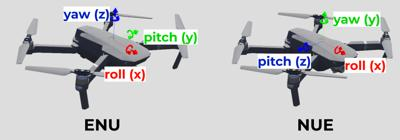
\includegraphics[width=0.8\textwidth]{figures/enu_nue.thumbnail.jpg}
    \caption{IMU-Knoten in Webots.}
    \label{fig:imu}
  \end{figure}
  
  \textbf{Rolle im Regelkreis:} Der IMU-Sensor bildet die zentrale \textbf{Rückführung} für die 
  \textbf{Balance-Regelung}. In jedem Simulationsschritt liest der PID-Regler 
  den aktuellen Rollwinkel $\varphi_{\text{roll}}$ aus der IMU und berechnet daraus 
  die Stellgröße für den Lenkantrieb. Konkret fungiert der Rollwinkel als 
  \emph{Regelgröße} im inneren Regelkreis: weicht das Fahrrad nach links/rechts ab, 
  soll durch einen entsprechenden Lenkeinschlag gegengesteuert werden, 
  bis $\varphi_{\text{roll}} = 0$ (senkrechte Lage) erreicht ist. Die hohe Abtastrate der IMU erlaubt es, den 
  \textbf{Regelkreis mit einer Zykluszeit von 2 ms} praktisch verzögerungsfrei zu schließen. 
  Dadurch reagiert der PID-Regler sehr schnell auf Lageänderungen, was eine Grundvoraussetzung ist, 
  um das instabile überhaupt beherrschen zu können. Im äußeren (vision-basierten) 
  Regelkreis spielt die IMU direkt keine Rolle, allerdings fließen die Balancierinformationen indirekt ein, wenn die Vision-Steuerung, 
  z.\,B. die Fahrgeschwindigkeit reduziert, sobald der Stabilitätsfaktor sinkt (starke Schräglage detektiert). 
  Insgesamt sorgt die IMU dafür, dass die \textbf{Regelstrecke} mit hoher Güte beobachtet wird, und bildet so das Fundament der Stabilisierung.


  Im C-Controller \texttt{balance\_control.c} wird die IMU über die Webots-API 
  initialisiert und ausgelesen. Listing~1 zeigt auszugsweise, wie das Gerät referenziert, 
  aktiviert und genutzt wird. Zunächst wird der Device-Tag der IMU mit ihrem Namen 
  \texttt{"imu"} angefordert und das Sensor-Sampling mit dem Simulationstimestep 
  (2~ms) eingeschaltet. In der Hauptschleife ruft der Regler dann kontinuierlich die Funktion 
  \texttt{wb\_inertial\_unit\_get\_roll\_pitch\_yaw()} auf, welche einen Vektor der Winkel zurückliefert. 
  Der Rollwinkel (Index 0 des Arrays) wird extrahiert und in die Regelung eingespeist. 
  Da die Webots-IMU per se idealisiert ist, entspricht dieser Winkel exakt der aktuellen 
  Fahrzeugneigung ohne Messfehler. Im Code ist dennoch ein Fallback vorgesehen: Falls der Supervisor-Knoten verfügbar ist, 
  wird alternativ dessen Orientierungs\-matrix ausgewertet – dies diente experimentell 
  der Verifikation der IMU-Daten und kann die gleiche Information liefern. 
  Im Normalfall nutzt der PID jedoch direkt die IMU-Daten. Der exemplarische Code zeigt, wie einfach die Orientierung in Webots abgefragt werden kann, 
  verglichen mit einer realen IMU (wo man per I\textsuperscript{2}C erst Rohdaten lesen und konvertieren müsste). 
  Die geringe Latenz der \texttt{wb\_inertial\_unit\_get\_roll\_pitch\_yaw}-Funktion 
  (nur ein Zeiger auf interne Simulationsdaten) trägt dazu bei, dass der Balance-Regelkreis 
  praktisch ohne zusätzliche Verzögerung arbeitet.


  \begin{lstlisting}[style=wbt,caption={IMU-Initialisierung und -Abfrage im C-Controller (Balance-Regelung)},label={lst:imu}]
    // IMU-Geraet initialisieren (in init_devices)
    imu_sensor = wb_robot_get_device("imu");
    wb_inertial_unit_enable(imu_sensor, timestep);  // Abtastrate = Welt-Zeitschritt (2 ms)
  
    // ... (im Hauptprogramm der Balance-Regelung)
  
    // Roll-, Pitch- und Gierwinkel vom IMU-Sensor abrufen
    const double *rpy = wb_inertial_unit_get_roll_pitch_yaw(imu_sensor);
    double roll_angle = rpy[0];  // aktueller Rollwinkel [Bogenmass]
  \end{lstlisting}
  


  %--------------------------------------------------
  % Kamera
  %--------------------------------------------------
  \subsubsection{Kamera (Videosensor)}

  \textbf{Physikalisches Prinzip:} Die Kamera dient als \textbf{optischer Sensor}, um die Strecke vor dem Fahrrad zu erkennen. Physikalisch basiert 
  sie auf einem \textit{digitalen Bildaufnehmer} (z.\,B. CMOS-Sensor), der durch eine Linse abgebildetes Licht in Pixelwerte umwandelt. In einem 
  realen System würde eine am Fahrzeug montierte Weitwinkel-Kamera laufend \textbf{Videobilder} der Fahrbahn liefern. Wesentliche Parameter sind 
  die \textbf{Auflösung} (Anzahl Pixel, bestimmt Detailgenauigkeit) und die \textbf{Bildrate} (Bilder pro Sekunde, bestimmt zeitliche Auflösung). 
  Für eine stabile Spurhaltung in Echtzeitanwendungen genügen in der Regel zweistellige Bildfrequenzen (\(\sim\!10\text{–}30\,\mathrm{Hz}\)), sofern 
  das Fahrzeug nicht extrem schnell fährt. Die Kamera erfasst visuelle Merkmale der Umgebung – im vorliegenden Kontext insbesondere die 
  \textbf{Straßenmarkierung} bzw. den Verlauf der Fahrspur – die dann von Bildverarbeitungsalgorithmen ausgewertet werden. Physikalisch können \textbf{Umgebungsfaktoren} wie Beleuchtung, 
  Bewegungsunschärfe oder Linsenverzerrungen die Bildqualität beeinflussen, was eine robuste \textbf{Merkmalsextraktion} herausfordernd macht. 
  Im Gegensatz dazu operiert eine Kamera jedoch \textbf{kontaktlos} und kann reichhaltige Umgebungsinformationen liefern, was sie ideal für die 
  \textbf{Pfadführung} macht (im Vergleich zu z.\,B. lokalen Sensorsignalen eines Gyroskops).



  \textbf{Simulation in Webots:} Webots simuliert Kameras über den \texttt{Camera}-Node, der virtuelle Renderings der 3D-Szene erzeugt. 
  Im \textit{Weltfile} ist für den Supervisor (die übergeordnete Instanz) eine Kamera mit definierter Position, 
  Ausrichtung und Eigenschaften eingebettet. Diese sogenannte \textit{Vision-Kamera} blickt aus erhöhter Perspektive 
  nach vorne unten auf die Fahrbahn (vergleichbar mit einer Helm- oder Drohnenkamera, die dem Fahrrad folgt).
  Die in der Simulation gewählte Auflösung beträgt z.\,B. 640$\times$360 Pixel bei einem Gesichtsfeld von ca. 
  114$^{\circ}$ (Field of View $\approx 2.0\,\mathrm{rad}$). Diese Einstellungen sind ein Kompromiss zwischen 
  Sichtfeld und Bilddetail – ein breites Sichtfeld erfasst die S-Kurve vollständig, während die moderate 
  Auflösung die Datenmenge und Rechenzeit begrenzt. Die Kamera liefert pro aktiviertem Zeitschritt ein Bild 
  im \textbf{RGBA-Format} (Rot–Grün–Blau plus Alphakanal) als Array von Byte-Werten.
  In der Controller-Software muss die Kamera explizit aktiviert werden, wobei die Abtastrate frei wählbar ist. 
  Der Vision-Controller nutzt eine Bildrate von rund 20~Hz, entsprechend einem Abtastintervall von 50~ms. 
  Dies ist deutlich langsamer als der Balance-Regelkreis, spiegelt aber die realistische Anforderung wider, 
  dass Bildverarbeitung zeitaufwändiger ist und nicht in jedem Simulationsschritt erfolgen muss. Im Webots-Code wird die Kamera z.\,B. mit 
  \texttt{camera.enable(50)} konfiguriert, sodass alle 50~ms ein neues Frame bereitgestellt wird. 
  Jedes Frame kann vom Controller über \texttt{camera.getImage()} abgeholt und weiterverarbeitet werden. 
  Zu beachten ist, dass Webots standardmäßig keine Kamerarausfälle oder Sensorschwächen simuliert – 
  die gelieferten Bilder sind idealisiert (scharf, bei gleichbleibender Beleuchtung). 
  Um Realismus zu erhöhen, könnten optional Rauschen oder Unschärfe simuliert werden; 
  im gegebenen Modell wird jedoch auf eine idealisierte Spurenerkennung abgezielt.

  \begin{figure}[H]
    \centering
    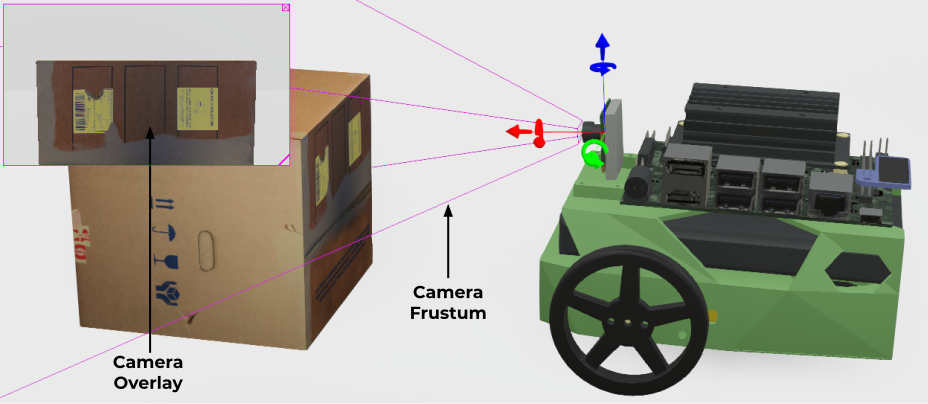
\includegraphics[width=0.8\textwidth]{figures/camera.png}
    \caption{Kamera-Knoten in Webots.}
    \label{fig:camera}
  \end{figure}


  \textbf{Rolle im Regelkreis:} Die Kamera ist der \textbf{Schlüsseleingang} für den vision-basierten äußeren Regelkreis. 
  Ihre Aufgabe besteht darin, dem \textbf{MPC-Fahrtrichtungsregler} Informationen über den Verlauf der Fahrspur 
  relativ zum Fahrzeug zu liefern. Im konkreten Szenario der S-Kurve extrahiert der Vision-Controller aus jedem Kamerabild 
  den lateralen Positionsfehler $e$ der Straße: also wie weit und in welche Richtung 
  das Fahrrad von der gewünschten Spurmitte abweicht. 

  Diese Bildverarbeitung geschieht in mehreren Schritten:


  \begin{enumerate}
    \item \textbf{Merkmalsextraktion:} Zunächst werden relevante Bildmerkmale berechnet, 
    etwa mittels \textbf{Segmentierung} der Straße. 
    Im Projekt wurde hierzu ein vortrainiertes YOLO-Modell verwendet, das die Fahrbahn in der Vogelperspektive segmentiert. 
    Falls kein KI-Modell verfügbar ist, greift ein Fallback auf klassische Bildverarbeitung: 
    Kantenerkennung und Auswertung eines definierten \textit{Region-of-Interest} liefern ebenfalls einen Schätzwert 
    für die Spurmittellage. 
    Ergebnis dieses Schritts ist der Querfehler $e$ (in normierter Form, z.\,B. $-0.5 \dots +0.5$ relativ zur Bildmitte) 
    sowie ggf. zusätzliche Qualitätskennzahlen (etwa die erkannte Kontur oder den Bedeckungsgrad der Fahrbahnmaske).
  
    \item \textbf{Spurführungsregelung:} Auf Basis des visuellen Fehlers bestimmt der Controller 
    einen passenden \textbf{Lenksollwert}. 
    Im entwickelten System kommt hierfür vorzugsweise ein 
    \textbf{modellprädiktiver Regler (MPC)} zum Einsatz, der das Fahrrad als dynamisches Modell 
    (Zustand $\mathbf{x} = [x,y,v,\psi]$) vorausberechnet. 
    Der MPC optimiert die Steuergröße Lenkwinkel $\delta$ (und ggf. Beschleunigung) 
    über einen kurzen Zeithorizont so, dass der Querfehler minimiert und 
    Fahrdynamikgrenzen (Lenkwinkel- und -ratenbegrenzung, Komfort) eingehalten werden. 
  
    Falls der MPC (etwa mangels Rechenpower) nicht verfügbar ist, 
    kann ersatzweise ein einfacherer PID-Ansatz verwendet werden (\textit{„Vision-PID“}), 
    der den Fehler $e$ in einen Lenkwinkel übersetzt. 
    In beiden Fällen resultiert ein Soll-Lenkwinkel $\delta_{\text{sol}}$ 
    bzw. ein normierter Lenkbefehl $u_{\text{vis}} \in [-1,1]$, 
    der an den Balance-Controller gesendet wird. 
  
    Zusätzlich kann die Vision-Einheit eine \textbf{Geschwindigkeitsempfehlung} $v_w$ berechnen – 
    z.\,B. wird bei großem Kurvenfehler eine niedrigere Fahrgeschwindigkeit empfohlen, 
    um die Stabilität zu wahren.
  \end{enumerate}

  \begin{figure}[H]
    \centering
    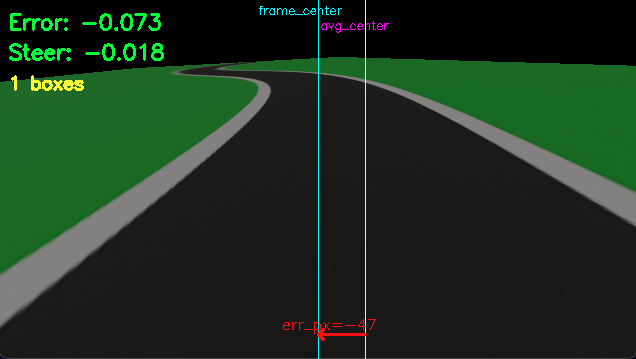
\includegraphics[width=0.8\textwidth]{figures/querfehler.png}
    \caption{Querfehler $e$ der Straße.}
    \label{fig:querfehler}
  \end{figure}

  Die Kamera beeinflusst den Balance-Regler auch indirekt, indem deren Messdaten 
  den \textbf{Kurs der Fahrt} vorgeben. 
  Wichtig ist, dass die Vision-Daten mit deutlich geringerer Frequenz ankommen als die IMU-Daten. 
  Der Balance-Controller hält während der 50~ms zwischen zwei Kamerabildern 
  die zuletzt empfangene Soll-Lenkvorgabe bei und stabilisiert weiterhin autonom. 
  Sobald ein neues Bild ausgewertet ist, wird der Lenksollwert ggf. korrigiert. Dieses \textbf{zweistufige Regelungskonzept} 
  (innere IMU-Schleife, äußere Vision-Schleife) 
  sorgt dafür, dass das Fahrrad einerseits aufrecht bleibt, andererseits aber auch aktiv 
  Richtungskorrekturen vornimmt, um einer kurvigen Referenzstrecke zu folgen. 
  Ohne die Kamera wäre nur ein statisches Balancieren oder eine Geradeausfahrt möglich – 
  erst der optische Sensor ermöglicht die \textit{spurtreue Autonomie} des Modells.

  %--------------------------------------------------
  % Motorsensoren (Inkrementalgeber)
  %--------------------------------------------------

  \subsubsection{Motorsensoren (Inkrementalgeber)}
  \textbf{Physikalisches Prinzip:} Neben IMU und Kamera, die den \textit{Zustand} des Fahrzeugs in Bezug auf Lage und Umwelt erfassen, 
  spielen sogenannte \textbf{Motorsensoren} eine wichtige Rolle für die interne Zustandsmessung. 
  Gemeint sind hier \textbf{Winkelgeber (Encoder)} an den drehbaren Komponenten – konkret am Lenkmotor und am Antriebsrad. 
  Physikalisch handelt es sich meist um \textit{inkrementelle Drehgeber}, 
  die auf der Motorachse montiert sind und pro Umdrehung eine bestimmte Anzahl Impulse (Zählschritte) liefern. 
  Durch Mitzählen der Impulse kann der Steuerrechner den zurückgelegten Winkel bestimmen; 
  über die Impulsfrequenz lässt sich auch die Drehgeschwindigkeit ermitteln. In echten Systemen werden beispielsweise \textbf{optische Encoder} (eine Scheibe mit Strichmuster und Fotodetektor) 
  oder \textbf{Hall-Sensoren} (Magnet und Hallsensor für Umdrehungszählung) eingesetzt. 
  Im Kontext unseres selbstbalancierenden Fahrrads wird der Lenkwinkel-Encoder benötigt, 
  um den aktuellen \textbf{Lenkeinschlag} zu kennen – wichtig etwa, um Lenkwinkelgrenzen nicht zu überschreiten 
  und für die protokollierte Ausgabe. 
  Der Hinterrad-Encoder erfasst die \textbf{Raddrehstellung} bzw. via Differenz auch die momentane Raddrehzahl, 
  was zur Abschätzung der Fahrgeschwindigkeit dient. 
  Physikalisch sind solche Sensoren sehr präzise (hochaufgelöste Encoder bieten $>1000$ Impulse/Umdrehung) 
  und liefern in schneller Abfolge Signale, typischerweise synchron zum Motor 
  (Erfassung erfolgt im kHz-Bereich, Latenzen sind vernachlässigbar). 
  Allerdings muss die Ansteuerungselektronik die Impulse auswerten (Interrupts zählen etc.), 
  was in der realen Implementierung zusätzlichen Programmieraufwand bedeutet.


  \textbf{Rolle im Regelkreis:} Die Positionssensoren werden vor allem zur \textbf{Überwachung und für abgeleitete Regelungsgrößen} genutzt. 
  Der \textbf{Lenkwinkelsensor} gibt dem Balance-Controller Feedback, welchen Lenkeinschlag der Motor aktuell realisiert – 
  dies ist nützlich, um z.\,B. einen \textit{Sättigungseffekt} zu erkennen: 
  Wenn der Soll-Lenkwinkel die mechanische Grenze erreicht, kann der Regler keine weitere Korrektur mehr bewirken. 
  Im Code wird aus dem Verhältnis von aktuellem Lenkausschlag zu Maximalwinkel ein \textbf{Stabilitätsfaktor} berechnet, 
  der als Indikator dient. 
  Außerdem fließt der gemessene Lenkwinkel in die Logging-Daten ein, 
  um das Reglerverhalten nachträglich analysieren zu können. Im laufenden Regler steckt der Lenkwert implizit schon in der Dynamik: 
  Da der Lenkmotor in Webots im Positionsmodus betrieben wird, sorgt das System automatisch dafür, 
  dass der Ist-Winkel dem Soll-Winkel folgt (siehe Abschnitt \textit{Aktuatoren}). 
  Ein separater Positionsregelkreis ist im Code also nicht implementiert – 
  im realen System würde hier ein unterlagerter Motor-PID am Encoder hängen, 
  aber in der Simulation übernimmt dies der Motorendpunkt. Der \textbf{Raddrehwinkelsensor} am Hinterrad wird primär genutzt, um die \textbf{Fahrgeschwindigkeit} zu ermitteln. 
  Im Controller-Code wird aus der zeitlichen Differenz des Radwinkels $\Delta \theta / \Delta t$ 
  die Winkelgeschwindigkeit $\omega$ berechnet und in km/h umgerechnet. 
  Diese Information kann für verschiedene Zwecke dienen: 
  einerseits zur \textbf{Ausgabe} (Anzeige der aktuellen Geschwindigkeit), 
  andererseits könnte sie in einen Geschwindigkeitsregler zurückwirken. Tatsächlich wird im Balance-Controller ein einfacher Speed-Controller benutzt, 
  der allerdings nicht die Ist-Geschwindigkeit, sondern den Vision-Lenkbefehl als Stellgröße nutzt 
  (d.\,h. bei starkem Lenken wird die Sollgeschwindigkeit reduziert). 
  Eine echte geschlossene Geschwindigkeitsregelung (Fahrgeschwindigkeit konstant halten) wäre ebenfalls denkbar – 
  hierzu würde der Rad-Encoder den Ist-Wert für einen Geschwindigkeits-PID liefern, 
  ähnlich wie im Hardware-Design mit Hall-Sensor beschrieben. Im aktuellen Simulationsmodell beschränkt sich die Nutzung also darauf, 
  \textbf{Zustandsgrößen} zu erfassen und die Regelung zu überwachen, weniger auf direkte Korrektur. 
  Dennoch sind die Encoder essenziell, um konsistente Zustandsinformationen zu haben: 
  z.\,B. ermöglicht der Radencoder dem System zu erkennen, ob das Fahrrad fährt oder fast steht, 
  was für die Balance eine Rolle spielen kann 
  (bei zu niedriger Geschwindigkeit nimmt die Selbststabilisierung ab).

  %--------------------------------------------------
  %--------------------------------------------------
  % Aktuatoren
  %--------------------------------------------------

  \newpage

  \subsection{Aktuatoren}
  Das selbstbalancierende Fahrradmodell verfügt über zwei zentrale \textbf{Aktuatoren}, 
  die als Stellglieder in die Dynamik des Systems eingreifen: 
  einen \textbf{Lenkantrieb} an der Vorderradgabel und einen \textbf{Antriebsmotor} für das Hinterrad. 
  Beide sind in Webots als \texttt{RotationalMotor}-Geräte realisiert und jeweils an einem drehbaren HingeJoint angebracht. 
  Physikalisch handelt es sich um \textbf{elektrische Rotationsmotoren} 
  (Gleichstrommotoren mit Getriebe), die in der Lage sind, Drehmomente aufzubringen 
  und so entweder einen bestimmten Winkel (Servomodus) oder eine bestimmte Drehgeschwindigkeit einzustellen. 
  Im Folgenden werden zunächst die realen Grundlagen dieser Aktuatoren betrachtet, 
  dann ihre Umsetzung in der Simulation und schließlich ihr konkreter Einsatz im Regelungssystem 
  mitsamt Code-Beispielen erläutert.

  \textbf{Physikalisches Wirkprinzip:} \\ 
  Bei \textbf{bürstenbehafteten DC-Motoren}, wie sie in vielen Robotikanwendungen Verwendung finden, 
  erzeugt ein stromdurchflossener Anker in einem Magnetfeld ein Drehmoment 
  (Lorentz-Kraftwirkung auf die Leiter). 
  Das resultierende \textbf{Motordrehmoment} ist annähernd proportional zum Ankerstrom, 
  während die Leerlauf-Drehzahl von der angelegten Spannung bestimmt wird. 
  Im offenen Regelkreis würde ein DC-Motor also schneller drehen bei höherer Spannung 
  und stärker drehen (mehr Kraft) bei höherem Strom. 

  Um präzise \textbf{Stellbewegungen} auszuführen, werden Motoren oft mit \textbf{Getrieben} 
  (zur Erhöhung von Drehmoment und Auflösung) und mit \textbf{Sensoren} rückgekoppelt (Encodern, s.\,o.). 
  So entsteht ein \textbf{Servoantrieb}: ein Motor-Getriebe-System mit interner Positions- oder Drehzahlregelung. 
  Im realen selbstbalancierenden Fahrrad gibt es zwei solcher Antriebe:
    
  \begin{itemize}
    \item \textbf{Der Lenkmotor} (z.\,B. ein Getriebemotor mit MD49-Motorcontroller) 
    verstellt den Lenkerwinkel. 
    Er arbeitet im Prinzip als \textbf{Positionsantrieb}: 
    auf einen Sollwinkel hin geregelt, mit einem begrenzten Arbeitsbereich (hier ca. $\pm 30^{\circ}$ mechanisch). 
    Der Motorcontroller nutzt den Encoder am Lenkgetriebe, um den Winkel exakt einzustellen 
    (geschlossener Regelkreis). 
    Physikalisch bedeutet dies, dass bei Abweichung zwischen Soll- und Ist-Winkel 
    ein proportional-integral-derivativer Korrekturstrom ins Motortreiber-Modul gegeben wird, 
    bis der Lenker die gewünschte Position erreicht. 
    Der Lenk­winkelantrieb muss schnell und kräftig genug sein, 
    um das Fahrrad innerhalb von Sekundenbruchteilen stabilisieren zu können – 
    in Jonah Zanders Hardware-Aufbau wurde z.\,B. ein starker 12\,V-Motor mit Untersetzung verwendet, 
    der $\pm 150^{\circ}$ in kurzer Zeit durchfahren kann.
  
    \item \textbf{Der Antriebsmotor} am Hinterrad (z.\,B. ein Nabenmotor oder kettengetriebener DC-Motor) sorgt für den Vortrieb. 
    Dieser wird im Unterschied zum Lenker meist als \textbf{Drehzahl- bzw. Drehmomentantrieb} betrieben. 
    Im realen System regelt man hier oft die Geschwindigkeit: 
    Ein separater PID hält die Raddrehzahl konstant, indem er den Motorstrom anhand des Hall-Encoder-Feedbacks justiert. 
    Physikalisch verleiht das rotierende Hinterrad dem System einen \textbf{gyroskopischen Effekt}, 
    der stabilisierend wirkt, weshalb eine gewisse Grundgeschwindigkeit hilfreich ist. 
    Gleichzeitig muss der Motor aber auch schnell drosseln oder bremsen können, 
    um Kurven sicher zu durchfahren, ohne umzukippen.
  \end{itemize}

  \newpage
  \textbf{Webots-Umsetzung:} Webots stellt mit dem \texttt{RotationalMotor}-Node einen Aktuator zur Verfügung, 
  der an einen HingeJoint gekoppelt Drehmomente ausüben kann. 
  Im Hintergrund berechnet der Physik-Kernel (ODE) die Wirkung des Motors auf das Gelenk 
  unter Berücksichtigung von Maximalmoment und Zielvorgabe. 
  Jeder Rotationsmotor kann in drei Modi betrieben werden:

    \begin{figure}[H]
      \centering
      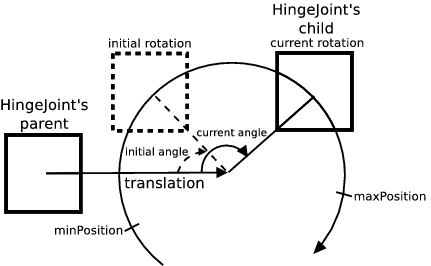
\includegraphics[width=0.6\textwidth]{figures/rotational_motor.png}
      \caption{Aktuatoren im Fahrradmodell.}
      \label{fig:aktuatoren}
    \end{figure}
    

  \begin{itemize}
    \item \textbf{Positionsmodus:} \\  
    Der Motor strebt einen vorgegebenen Zielwinkel an (\texttt{setPosition(angle)}), 
    wobei er innerhalb der konfigurierten Kraft- und Geschwindigkeitsgrenzen das nötige Drehmoment erzeugt, 
    um diesen Winkel zu erreichen. Dieser Modus entspricht einem Servomechanismus.  
    Im Webots-Modell ist der Lenkungsaktor in den Positionsmodus geschaltet.  
    Dazu wird im Code einmalig 
    \texttt{wb\_motor\_set\_position(handlebars\_motor, 0.0)} 
    aufgerufen, um die Start-Sollposition (geradeaus) zu setzen.  
    Anschließend erhält der Lenkmotor in jeder Regeliteration einen neuen Sollwinkel.  
    Die Regelung der Position übernimmt Webots intern: 
    der Motor wirkt wie eine Feder-Dämpfer-Kopplung ans Gelenk, 
    die Differenz zwischen Ist- und Sollwinkel generiert ein entsprechendes Gegendrehmoment (virtueller P-Regler).  
    Parameter wie \texttt{maxTorque} und \texttt{maxVelocity} im Weltfile bestimmen, 
    wie schnell und kräftig das Soll nachgeführt wird.  
    Im Modell sind z.\,B. für den Lenkmotor \texttt{maxTorque = 25\,Nm} festgelegt – 
    ein Wert, der sicherstellt, dass genügend Kraft zum Aufrichten aus Schräglagen vorhanden ist, 
    ohne das System zu unrealistisch zu machen.

    \item \textbf{Geschwindigkeitsmodus:} \\  
    Hier wird dem Motor eine Ziel-Angulargeschwindigkeit vorgegeben (\texttt{setVelocity(omega)}), 
    während die Position auf unendlich gesetzt wird (\texttt{setPosition(INFINITY)}).  
    In Webots bedeutet dies, dass der Motor keinen festen Endwinkel hat, sondern kontinuierlich dreht.  
    Der Antriebsmotor des Hinterrads wird so betrieben: 
    im Initialisierungscode wird \texttt{wb\_motor\_set\_position(wheel\_motor, INFINITY)} 
    aufgerufen, was den Wechsel in den Geschwindigkeitsmodus bewirkt.  
    Fortan interpretiert Webots den Befehl \texttt{wb\_motor\_set\_velocity(wheel\_motor, v)} 
    als Soll-Drehzahl (in Rad/s) für das Rad.  
    Intern wirkt wieder ein virtueller Regler, der das nötige Drehmoment aufbringt, 
    um diese Geschwindigkeit zu erreichen/halten (bis zum max. Drehmoment).  
    Im Weltmodell ist für den Hinterradmotor ein recht hohes maximales Drehmoment von 120\,Nm erlaubt, 
    um Beschleunigungsvorgaben schnell umsetzen zu können.  
    Allerdings ist die erreichbare Drehzahl in der Praxis auch durch die Antriebsspannung bzw. Webots-Parameter 
    \texttt{maxVelocity} limitiert.  
    In S-Kurven-Simulationen wurde typischerweise eine Grundgeschwindigkeit von ca. $3$–$5\,\mathrm{m/s}$ gefahren, 
    was durch den entsprechenden \texttt{velocity}-Wert in Rad/s vorgegeben wird.
    \item \textbf{Kraft-/Drehmomentmodus:}  
    Alternativ kann man in Webots Motoren auch direkt ein Drehmoment vorgeben 
    (\texttt{setTorque(t)}), um z.\,B. eigene Regelalgorithmen für die Positions- und Geschwindigkeitssteuerung umzusetzen.  
    In unserem Modell wird dieser Modus nicht explizit genutzt, 
    da die beiden in Steuerungsmodellen gängigen Modi bereits ausreichen.  
    Dennoch ist es wichtig zu wissen, dass Webots stets mit Kräften/Momenten rechnet: 
    Die Position- und Velocity-Modelle setzen letztlich ein solches Drehmoment um, 
    das aus der jeweiligen Referenzgröße berechnet wird.
  \end{itemize}


  Die beiden Motoren sind im Weltfile als Geräte \texttt{handlebars motor} und 
  \texttt{motor::wheel} deklariert und jeweils dem passenden HingeJoint zugeordnet. 
  Webots erlaubt es, mehrere Motoren pro Gelenk zu definieren, 
  doch hier ist jeweils nur einer aktiv. 

  Die Namensgebung \texttt{motor::wheel} für den Hinterradantrieb ist ein Spezialfall: 
  Das Präfix \texttt{::} dient dazu, den Motor vom gleichnamigen (per DEF) vorderen Rad zu unterscheiden, 
  welches ebenfalls als \texttt{wheel} benannt ist – so können Kollisionen in der Namensauflösung vermieden werden. 
  Im Controller-Code greift man dann genau mit diesem Namen zu.

  \subsubsection*{Rolle im Regelkreis}

  Die Aktuatoren setzen die vom Regler berechneten Sollgrößen in physikalische Bewegung um 
  und schließen damit die \textbf{Wirkkette des Regelkreises}. 
  Konkret berechnet der Balance-Controller in jedem Zeitschritt zwei Stellwerte:

  \begin{itemize}
    \item den \textbf{Lenksollwinkel} $\delta_{\text{sol}}$ 
    (aus dem PID-Regler + Vision-Überlagerung), und
    \item die \textbf{Antriebs-Sollgeschwindigkeit} $v_{\text{sol}}$.
  \end{itemize}

  Diese Sollwerte werden direkt an die Motoren übergeben. 
  Der Lenkwinkel-Sollwert stammt aus der Kombination des inneren und äußeren Regelkreises: 
  Wie in Abschnitt \textit{Sensoren} erläutert, fusioniert der Controller den 
  \textbf{Balance-Anteil} (zur Selbstausrichtung) mit dem \textbf{Vision-Anteil} 
  (zur Kurvenfahrt) zu einer endgültigen Vorgabe \texttt{final\_steer}. 
  Dieses \texttt{final\_steer} entspricht einem Winkel in Radiant, 
  der begrenzt auf den physikalisch möglichen Bereich ($\pm 0.524$\,rad) 
  an den Lenkmotor geschickt wird. 

  Der Hinterrad-Sollwert \texttt{target\_speed} wird ebenfalls bestimmt – 
  im aktuellen Konzept abhängig vom Lenkeinschlag 
  (starker Lenkeinschlag $\rightarrow$ automatische Reduktion der Grundgeschwindigkeit). 
  Damit fungiert der Balance-Controller gleichzeitig als einfacher 
  \textbf{Geschwindigkeitsmanager}, 
  der z.\,B. in Kurven abbremst, um die Balance nicht zu gefährden. 
  Die Berechnung von \texttt{target\_speed} erfolgt durch einen separaten Algorithmus 
  (\texttt{speed\_pid\_compute}), 
  der den Vision-Lenkbefehl in eine prozentuale Reduktion der Grundgeschwindigkeit umsetzt. 
  Alternativ könnte hier ein echtes Geschwindigkeits-PID auf Basis der Encoder-Daten stehen – 
  dies ist eine mögliche Erweiterung. 

  Sobald die Stellgrößen vorliegen, werden sie an die Motor-API übergeben. 
  Damit findet die \textbf{Regler-Ausgabe} statt: 
  Die Software schreibt die Sollwerte in die Motoren, 
  und die Physiksimulation reagiert, indem sie die entsprechenden Kräfte auf das Modell einleitet. 

  Der \textbf{Lenkmotor} dreht die Vorderradgabel proportional zum Regelfehler – 
  wenn das Fahrrad z.\,B. nach rechts kippt (positiver Rollwinkel), 
  verlangt der PID einen Lenkeinschlag nach rechts, 
  um einen stabilisierenden Lenkimpuls zu erzeugen 
  (das Rad wird unter den Schwerpunkt gesteuert, ähnlich wie man einen fallenden Besen durch Vorziehen stabilisiert). 
  Gleichzeitig berücksichtigt der Vision-Anteil, ob ggf. bewusst in eine Kurve gelenkt werden soll. 
  Die resultierende Motorbewegung ist somit eine Überlagerung aus Stabilisieren und Navigieren. 

  Der \textbf{Hinterradmotor} liefert währenddessen den Vortrieb: 
  Eine Grundgeschwindigkeit hält das Fahrrad in Bewegung 
  (was das Balancieren erleichtert, da dynamische Stabilisierungskräfte wirken), 
  und bei Bedarf wird verlangsamt. 
  Im Geradeausfall (Vision inaktiv) regelt der Balance-Controller sogar nur die Balance 
  und reduziert Geschwindigkeit auf ein Mindestmaß, falls keine Steuerkommandos kommen. 

  Insgesamt sorgen die Aktuatoren dafür, 
  dass die vom Regler vorgegebenen Stellgrößen (Lenkwinkel, Antriebskraft) 
  tatsächlich umgesetzt werden – 
  sie sind somit die finalen Ausführungselemente des Reglers. 
  Ohne ausreichende Aktuatorleistung könnte das beste Regelgesetz das Fahrrad nicht stabilisieren; 
  in der Simulation sind sie jedoch so gewählt, dass die Anforderungen erfüllt werden.

  \textbf{Implementierung und Code-Integration:} Die Ansteuerung der Motoren erfolgt im Balance-Controller (C-Code) nach Berechnung der Sollwerte. 
  Bereits während der Initialisierung werden die Motoren konfiguriert: 
  Listing~4 zeigt, wie der Lenkmotor und der Radmotor als Devices geholt und in die gewünschten Modi versetzt werden. 
  Für den Lenkantrieb wird die Position initial auf $0.0$ gestellt (\textit{Lenker gerade}). 
  Für den Hinterradantrieb wird \texttt{wb\_motor\_set\_position(wheel\_motor, INFINITY)} gesetzt, 
  was – wie oben beschrieben – den Geschwindigkeitsmodus aktiviert. 
  Beide Motoren würden standardmäßig mit \texttt{velocity = 0} starten; 
  der Hinterradmotor erhält später im laufenden Betrieb eine Startgeschwindigkeit (Basiswert). 

  Im Regelprozess selbst (Hauptschleife) werden dann die aktuellen Stellbefehle übergeben:

  \begin{lstlisting}[language=C,caption={Motorsteuerung im Regelkreis},label={lst:motorsteuerung}]
  wb_motor_set_position(handlebars_motor, -final_steer);
  wb_motor_set_velocity(wheel_motor, target_speed);
  \end{lstlisting}

  Dabei ist wichtig zu erwähnen, dass der Lenkwinkel mit negativem Vorzeichen gesetzt wird. 
  Dies rührt von der Achsdefinition her – je nach Koordinatensystem ist eine positive Rotation der Lenkachse evtl. 
  als Linkseinschlag definiert, während der Regler positive Werte als Rechtsdrehung interpretiert (oder umgekehrt). 
  Durch das Vorzeichen wird sichergestellt, dass z.\,B. ein positiver Reglerausgang 
  (Korrektur nach rechts) tatsächlich den Lenker nach rechts steuert. 
  Solche Vorzeichenkonventionen sind in der Modellierung zu beachten. 

  Der Wert \texttt{target\_speed} wird in Rad/Sekunde an das Hinterrad übergeben. 
  Um einen Eindruck zu geben: Eine Zielgeschwindigkeit von z.\,B. 4\,m/s entspricht 
  (bei $\sim$0.7\,m Raddurchmesser) ungefähr 11.4\,rad/s Winkelgeschwindigkeit. 

  Das Logging im Code zeigt typischerweise Werte um 10–15\,rad/s für die Grundgeschwindigkeit. 
  Nachdem die Sollwerte gesetzt sind, greift die Webots-Physik die neuen Sollwerte im nächsten Zeitschritt auf 
  und beschleunigt/verstellt die Motoren entsprechend. 
  Im Code werden nach dem Setzen der Motoren noch Statuspakete versendet und Logging betrieben, 
  was für die Aktuatorwirkung selbst aber keine Rolle mehr spielt.



  Insgesamt ist die Motoransteuerung in Webots sehr direkt – ein Funktionsaufruf genügt, 
  um das physikalische Stellglied zu beeinflussen. 
  Dies erlaubt es, die Regelalgorithmen unkompliziert mit der Simulationswelt zu koppeln. 
  Listing~4 fasst die wichtigsten Schritte zusammen. 
  Hier sind sowohl die Initialisierung (Modussetzen) als auch die Laufzeitschleifen der Motoren zu sehen, 
  mit deutschen Kommentaren erläutert. 
  Man erkennt, wie die Aktuator-Schnittstelle an die zuvor beschriebenen Regelungsgrößen gebunden ist: 
  \texttt{final\_steer} (in rad) geht an den Lenkmotor, 
  \texttt{target\_speed} (in rad/s) an den Radmotor. 
  Diese Werte stammen direkt aus der Regelung (siehe vorherigen Abschnitt) – 
  es findet keine weitere Transformation mehr statt, da die Größeneinheiten 
  konsistent mit dem Webots-Modell gewählt wurden.
  
  \begin{lstlisting}[style=wbt_c,caption={IMU-Initialisierung und -Abfrage im C-Controller (Balance-Regelung)},label={lst:imu3}]
    // Motoren-Devices abrufen
    handlebars_motor = wb_robot_get_device("motor::handlebars");
    wheel_motor     = wb_robot_get_device("motor::wheel");
    if (handlebars_motor == 0 || wheel_motor == 0) {
        exit(1);
    }
    // Initialisierung der Motoren
    // Lenkmotor: Positionsmodus, Startwinkel = 0 rad
    wb_motor_set_position(handlebars_motor, 0.0); 
    // Hinterradmotor: Geschwindigkeitsmodus aktivieren
    wb_motor_set_position(wheel_motor, INFINITY);    
    // (Velocity bleibt zunaechst 0, wird spaeter gesetzt)
    
    //...(im Reglerloop, nach PID/MPC-Berechnung von final_steer/target_speed)
    
    // Lenkantrieb: Soll-Lenkwinkel setzen 
    wb_motor_set_position(handlebars_motor, -final_steer); 
    // Radantrieb: Soll-Drehgeschwindigkeit setzen
    wb_motor_set_velocity(wheel_motor, target_speed);      
 
  \end{lstlisting}
  

  Durch diese Implementierung wird das Zusammenwirken aller Komponenten deutlich: 
  \textbf{Sensoren} (IMU, Kamera, Encoder) liefern den aktuellen Zustand, 
  der \textbf{Regler} (PID \& MPC) berechnet daraus Stellgrößen, 
  und die \textbf{Aktuatoren} (Motoren) führen diese Stellgrößen am physikalischen Modell aus. 
  Die Webots-Simulation ermöglicht es, all dies in einem deterministischen Umfeld zu testen – 
  etwaige Fehlanpassungen (wie zu schwache Motoren oder unzureichende Sensorfrequenzen) 
  würden sofort im Verhalten sichtbar und könnten iterativ justiert werden, 
  bevor der Algorithmus auf einen realen Prototyp übertragen wird.



  \subsection{Controller}


  Ein Webots\mbox{-}Controller ist ein separates Programm (Prozess), das einen Roboter in der Simulation steuert 
  und über eine definierte API mit der Simulationswelt kommuniziert. Für jeden Roboter kann ein Controller in 
  C/C++, Python, Java oder MATLAB laufen, wobei Webots den Datenaustausch (Sensorwerte, Aktuatorbefehle) bei 
  jedem Simulationsschritt synchronisiert. Typischerweise durchläuft ein Controller eine Endlosschleife, in 
  der er Sensoren liest, Berechnungen durchführt und Aktuatoren ansteuert, wobei am Ende jeder Iteration die 
  Funktion \texttt{wb\_robot\_step()} aufgerufen werden muss. Dieser Aufruf übergibt die gewünschte 
  Control\mbox{-}Step\mbox{-}Dauer (in Millisekunden) an den Simulator und bewirkt, dass Webots die 
  Simulation um genau diesen Zeitschritt fortsetzt und dabei alle bis dahin vom Controller gesetzten 
  Befehle anwendet. Danach erhält der Controller die aktualisierten Sensorwerte des neuen Simulationszustands 
  zurück. Abbildung~3.6 veranschaulicht diese Synchronisation \cite{cyberbotics_controller_programming}.
  
  \begin{wrapfigure}{r}{0.5\textwidth} % r=rechts, l=links
    \vspace{-0.8\baselineskip}          % optional: nach Bedarf anpassen
    \centering
    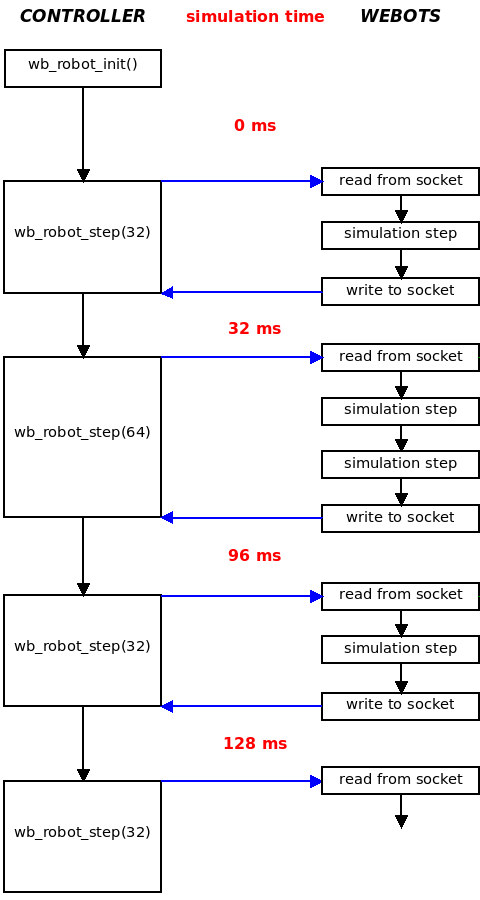
\includegraphics[width=\linewidth]{figures/controller_synchronization.png}
    \caption{Synchronisation zwischen Controller und Simulation.}
    \label{fig:controller_sync}
  \end{wrapfigure}


  Alle Anweisungen vor dem nächsten Zeitschritt (\texttt{wb\_robot\_step}\mbox{-}Aufruf) werden zunächst gesammelt; 
  mit dem Step\mbox{-}Aufruf rechnet der Simulator den nächsten Physikschritt und aktualisiert die Sensoren, bevor 
  der Controller weiterläuft. Auf diese Weise laufen Simulation und Controller \emph{synchron} in gleichmäßigen
   Zeitschritten. Standardmäßig wartet Webots in diesem synchronen Modus darauf, dass jeder Controller seinen \texttt{wb\_robot\_step} 
  ausführt, bevor der nächste Simulationsschritt erfolgt. Dies garantiert Konsistenz, erlaubt aber auch differierende Abtastraten: 
  Der Kontrollschritt muss ein ganzzahliges Vielfaches des Simulations\mbox{-}Basisschritts sein.

  Beispielsweise kann bei einer Weltzeit-schrittauflösung von 2\,ms ein Controller mit 2\,ms, 10\,ms oder 50\,ms 
  Schrittweite betrieben werden — Webots führt dann pro Controller-schritt entsprechend 1, 5 bzw.\ 25 Simulationsschritte 
  aus und wartet am Ende ggf.\ auf den Controller. Diese Entkopplung nutzt Webots, um auch langsamere Controller (z.\,B.\ in Python) 
  in eine schnelle Physiksimulation einzubetten, ohne die Synchronisation zu verlieren.

  Um auf Sensoren und Aktuatoren zuzugreifen, stellt Webots gerätespezifische API\mbox{-}Funktionen bereit. Im C\mbox{-}Controller 
  werden z.\,B.\ Geräte über \texttt{wb\_robot\_get\_device("name")} referenziert und Sensoren mit \texttt{wb\_sensor\_enable()} 
  aktiviert. Entsprechende Methoden existieren in Python (\texttt{robot.getDevice()}, \texttt{device.enable()}). Ein Sensor liefert 
  erst ab dem nächsten \texttt{wb\_robot\_step()} gültige Messwerte, da die Simulationszeit dann fortgeschritten ist. 

  Aktuatorbefehle (z.\,B.\ \texttt{wb\_motor\_set\_position()} oder \texttt{motor.setPosition()} in Python) werden zunächst lokal 
  gepuffert—die tatsächliche Ausführung in der Physik\mbox{-}Engine erfolgt erst am nächsten Step\mbox{-}Synchronisationspunkt. Daher 
  ist es sinnlos, in derselben Schleifeniteration zwei unterschiedliche Positionen für denselben Motor zu setzen: Nur der zuletzt vor 
  \texttt{wb\_robot\_step()} gesetzte Wert wird im kommenden Schritt ausgeführt. Ebenso bleiben zwei unmittelbar nacheinander gelesene 
  Sensorsamples identisch, solange kein Simulationsschritt dazwischen liegt. Dieses deterministische Schritt\mbox{-}für\mbox{-}Schritt\mbox{-}
  Ausführungsmodell erleichtert die Reproduzierbarkeit und verhindert \emph{race conditions} zwischen Physik und Reglercode.

  Für das selbstbalancierende Fahrrad wurden zwei Controller\mbox{-}Prozesse implementiert, die in Webots zeitgleich laufen und 
  über die oben beschriebene Mechanik gekoppelt sind: Einerseits der \emph{Balance\mbox{-}Controller} auf dem Fahrrad (in C, hoher Takt), 
  andererseits ein \emph{Vision\mbox{-}Controller} auf einem Supervisor\mbox{-}Knoten (in Python, langsamer Takt). Die Welt ist so 
  konfiguriert, dass das Fahrrad einen \texttt{Receiver} und einen \texttt{Emitter} trägt, während der Supervisor das komplementäre 
  Gegenstück besitzt; damit entsteht ein bidirektionaler Nachrichtenkanal innerhalb der Simulation:

  \begin{lstlisting}[style=wbt_c,caption={Nachrichtenkanal zwischen Controller und Simulation},label={lst:imu4}]
    Robot {
      Controller "balance_control_c"
      Receiver { name "command_rx"  channel 1  bufferSize 64 }
      Emitter  { name "status_tx"   channel 2  bufferSize 64 }
    }
    Supervisor {
      Controller "vision_control_py"
      Emitter  { name "command_tx"  channel 1  bufferSize 64 }
      Receiver { name "status_rx"   channel 2  bufferSize 64 }
    }
  \end{lstlisting}

  Über Channel 1 sendet der Vision-Controller Steuerkommandos an das Fahrrad, 
  und über Channel 2 übermittelt der Balance-Controller seinerseits Statusdaten zurück (z.\,B.\ aktueller Rollwinkel, Lenkwinkel, 
  Geschwindigkeit). Beide Controller laufen im \emph{synchronen Modus}, d.\,h.\ Webots hält die Physik so lange an, bis sowohl der 
  schnelle C-Controller (alle 2\,ms) als auch der langsamere Python-Controller ihren Schritt abgearbeitet haben \cite{cyberbotics_emitter}\cite{cyberbotics_receiver}. 
  Praktisch bedeutet dies: Der Balance\mbox{-}Regler berechnet bei jedem Simulationsschritt neue Motorbefehle, während der
  Vision\mbox{-}Algorithmus nur alle 25 Schritte (50\,ms) ein neues Lenkkommando liefert. Die folgenden Punkte fassen Aufgaben und Interaktion zusammen:

  \begin{itemize}
    \item \emph{Balance\mbox{-}Controller (C, 500\,Hz):} Liest hochfrequent IMU\mbox{-} (Rollwinkel) und Radsensoren aus, regelt 
    den Balancierwinkel mittels PID und steuert den Lenkmotor sowie den Antriebsmotor kontinuierlich an. Verarbeitet eingehende Sollkommandos 
    der Vision\mbox{-}Ebene (z.\,B.\ Lenkwinkel) und kombiniert sie mit dem internen Regleroutput. Sendet zyklisch seinen Status 
    (Stabilitätsmaß, aktuelle Geschwindigkeit etc.) über den Emitter aus. Bei Ausbleiben externer Kommandos hält er das Fahrzeug 
    selbständig im Gleichgewicht (Fallback auf reinen Balance\mbox{-}Modus).
    \item \emph{Vision\mbox{-}Controller (Python, \(\sim\)20\,Hz):} Läuft als Supervisor\mbox{-}Controller mit Zugriff auf globale 
    Informationen. Nutzt die am Fahrzeug montierte Kamera (Bildrate ca.\ 20\,Hz) zur Fahrbahnerkennung (z.\,B.\ YOLO\mbox{-}Segmentierung) 
    und berechnet auf dieser Basis einen Trajektorien\mbox{-} bzw.\ Lenksollwert mittels modellprädiktiver Regelung (MPC) oder wahlweise 
    eines PID. Dieses Sollkommando wird paketbasiert an den Balance\mbox{-}Controller gesendet (\texttt{Emitter} auf Kanal 1). Zudem 
    überwacht der Vision\mbox{-}Controller den empfangenen Fahrzeugzustand (\texttt{Receiver} auf Kanal 2), um die Regelgüte zu 
    beurteilen oder Logging durchzuführen. Gegebenenfalls passt er seine Fahrstrategie an (etwa Geschwindigkeitsanpassung bei großen Balance\mbox{-}Fehlern).
  \end{itemize}

  Durch diese Aufteilung konnte eine zweistufige Regelungsarchitektur realisiert werden: Der innere C\mbox{-}Regler stabilisiert 
  das Fahrrad auf kurzen Zeitskalen autonom, während der äußere Python\mbox{-}Regler in größeren Abständen Kurskorrekturen vorgibt. 
  Webots gewährleistet die Synchronisierung beider Teilprozesse, sodass Kommandos verlustfrei und deterministisch am 
  Step\mbox{-}Synchronisationspunkt ausgetauscht werden. Im Ergebnis reagiert das Gesamtsystem echtzeitnah auf Störungen 
  (Balance) und plant zugleich vorausschauend seine Fahrtrajektorie; die Kopplung konnte in der Simulation umfassend getestet 
  und für den späteren Hardware\mbox{-}Einsatz vorbereitet werden.




  \subsection{Angebundene GUI}


  Die Simulationsumgebung verfügt über ein tkinter\mbox{-}basiertes GUI\mbox{-}Kontrollzentrum, mit dem sich die Regelungsparameter 
  des selbstbalancierenden Fahrrads in Echtzeit anpassen und die Fahrdaten live überwachen lassen. Dieses GUI bietet eine benutzerfreundliche 
  Oberfläche, um während der laufenden Webots\mbox{-}Simulation Einstellungen zu ändern, ohne die Simulation unterbrechen zu müssen. 
  Es gliedert sich in mehrere Tabs, von denen insbesondere \enquote{Parameter} und \enquote{Monitoring} für die Laufzeitanpassung 
  und \mbox{-}beobachtung relevant sind. Im Folgenden wird erläutert, wie diese Tabs funktionieren und wie die Laufzeitanpassung 
  der Parameter sowie das Live\mbox{-}Monitoring umgesetzt sind.


  \textbf{Parameter-Tab \mbox{-} Laufzeitfähige Parameteranpassung:} Der Parameter\mbox{-}Tab ermöglicht die direkte Einstellung der Regelungsparameter während der Simulation. Über Slider und 
  Eingabefelder können z.\,B.\ PID\mbox{-}Reglergrößen (Kp, Ki, Kd) und andere Steuerungsgrößen komfortabel angepasst werden. Dabei werden die aktuellen Werte in Echtzeit im GUI angezeigt 
  und validiert, während der Nutzer sie ändert. Einzelne Parametergruppen (etwa Winkel\mbox{-}PID, Geschwindigkeitsregelung, mechanische Limits) 
  sind übersichtlich gruppiert, sodass man nicht auf die Details jedes Parameters eingehen muss, aber einen strukturierten Überblick behält.

  Wesentlich ist, dass Änderungen unmittelbar wirksam werden, ohne die Simulation neu zu starten. Technisch geschieht dies durch ein 
  SON\mbox{-}basiertes Konfigurationssystem im Hintergrund. Das GUI lädt zu Beginn die aktuellen Parameter aus einer Konfigurationsdatei 
  (z.\,B.\ \texttt{balance\_config.json}) und schreibt geänderte Werte bei Bedarf zurück. Wird ein Wert verändert, kann der Nutzer die 
  neue Konfiguration speichern und anwenden (Schaltflächen \enquote{Speichern} bzw.\ \enquote{Anwenden} im GUI). Die laufende 
  Regelungssoftware erkennt diese Aktualisierung dank eines Hot\mbox{-}Reload\mbox{-}Mechanismus: Der Balance\mbox{-}Controller 
  lädt die JSON\mbox{-}Config in kurzen Intervallen oder auf Befehl neu, sodass geänderte Parameter sofort in den Regler einfließen.


  \textbf{Monitoring-Tab – Live-Datenvisualisierung und CSV-Logging: }Im \emph{Monitoring}-Tab werden Fahr- und Regeldaten \emph{live} visualisiert, 
  um das Verhalten des Fahrrads während der Simulation nachvollziehen zu können. Abbildung 9 zeigt den Monitoring-Tab mit Echtzeitdiagrammen. 
  Der Tab bietet interaktive Plots, die zentrale Größen über der Zeit darstellen — etwa den Rollwinkel, den Lenkausgang des Reglers, die aktuelle 
  und Ziel-Geschwindigkeit sowie die PID-Regleranteile (P, I, D). Über Auswahlkästchen kann gezielt gesteuert werden, welche Kurven angezeigt werden, 
  um den Überblick zu behalten; beispielsweise lassen sich nur die Balance-Controller-Daten oder nur die PID-Terme ein- oder ausblenden. Zusätzlich 
  stehen Zoom-Regler zur Verfügung, um den dargestellten Zeitraum einzugrenzen und Details zu analysieren.

  Die Datengrundlage bilden CSV-Protokolldateien, die vom Balance-Controller während jeder Fahrt automatisch erzeugt werden. Jede Simulation 
  (bzw.\ Fahrt) wird lückenlos in einer Log-Datei festgehalten — mit Zeitstempel und den relevanten Mess- und Steuergrößen (u.\,a.\ Winkel, 
  Geschwindigkeiten, Reglerausgänge, Fehlerwerte). Der Monitoring-Tab listet diese Aufzeichnungen und ermöglicht sowohl das nachträgliche Laden 
  einer aufgezeichneten CSV-Datei als auch den Live-Stream der jeweils neuesten Datei. Im Live-Modus wählt das System automatisch die aktuell 
  von der Simulation beschriebene Log-Datei aus und aktualisiert die Plots fortlaufend; alternativ kann der Benutzer eine frühere Aufzeichnung 
  vollständig laden und visualisieren. In beiden Fällen normalisiert das GUI die eingelesenen CSV-Daten (z.\,B.\ Umrechnung von Radmaß in Grad 
  oder m/s in km/h) und zeichnet zweigeteilt: typischerweise erscheinen Winkel- und Lenkdaten im oberen Diagramm, die PID-Terme sowie Geschwindigkeiten 
  im unteren, jeweils mit gemeinsamer Zeitachse.
  \begin{figure}[H]
    \centering
    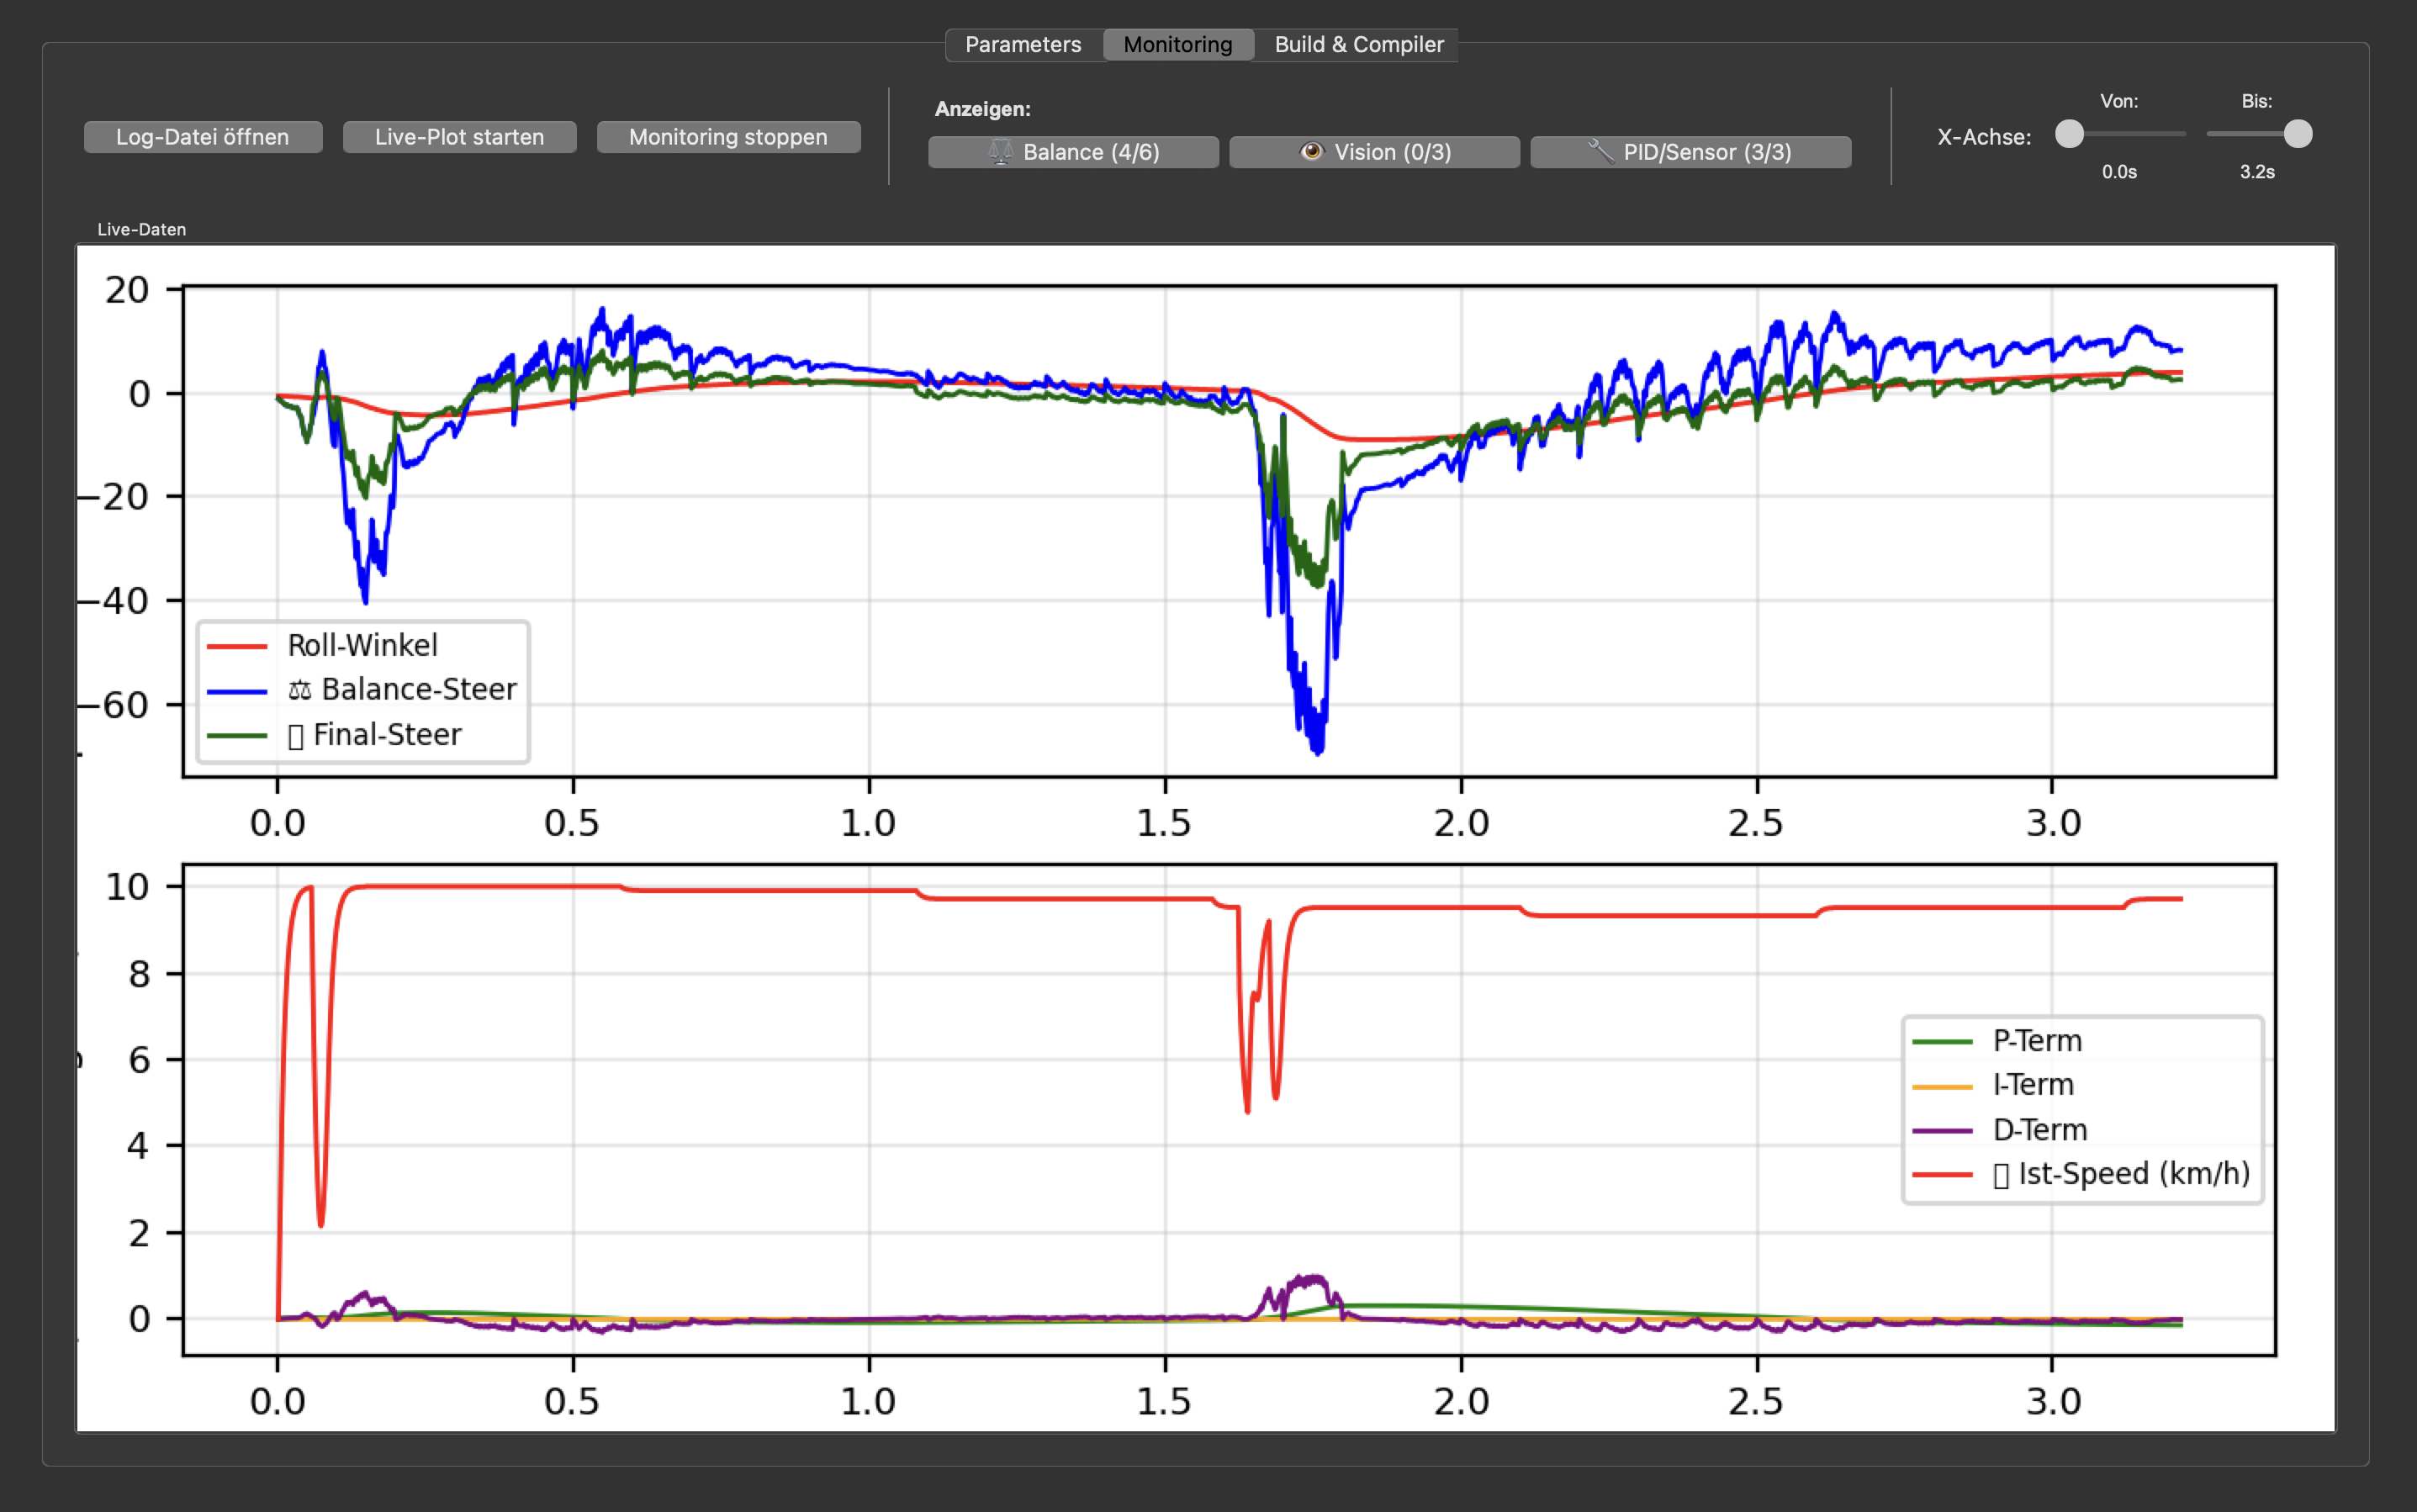
\includegraphics[width=1.0\textwidth]{figures/GUI_2.png}
    \caption{Monitoring-Tab mit Echtzeitdiagrammen.}
    \label{fig:GUI_2}
  \end{figure}

  Ergänzend zur grafischen Darstellung bietet der Monitoring-Tab Statusanzeigen, die u.\,a.\ den aktuell geladenen Logfile-Namen, den Zeitpunkt 
  der letzten Aktualisierung und den Laufzustand des Controllers ausweisen. So bleibt stets transparent, ob die Verbindung zur Simulation aktiv 
  ist und welche Datenquelle visualisiert wird. Zusammengenommen stellt der Monitoring-Tab ein leistungsfähiges Werkzeug dar, um die Auswirkungen 
  von Parameteränderungen sofort sichtbar zu machen und das Systemverhalten mittels aufgezeichneter Daten zu analysieren. Die Kombination aus
  laufzeitfähiger Parameteranpassung und Live-Monitoring ermöglicht ein effizientes Trial-and-Error-Tuning des selbstbalancierenden Fahrrads, 
  unterstützt durch intuitive GUI-Interaktion und automatisierte Datenaufzeichnung.

 





